\documentclass{assignment}
\UsingEnglish
\ProjectInfos*{Intro to Communication System}{EE140}{Fall, 2020}{Assignment 3}{Due time : 10:15, Oct 9, 2020 (Friday)}{陈稼霖}{45875852}
\begin{document}
\begin{prob}[Autocorrelation and cross-correlation function, 30 pts]
    The random process are given by $X(t)=n(t)+A\cos(2\pi f_0t+\theta)$, $Y(t)=n(t)+A\sin(2\pi f_0t+\theta)$, where $A$ and $f_0$ are positive constants and $\theta$ is a random variable uniformly distributed in the interval $[-\pi,\pi)$. The first term $n(t)$ represents a stationary random noise process with autocorrelation function $R_n(\tau)=B\Lambda(\tau)+C$, where $B$ and $C$ are positive constants. We further assume the random process $n(t)$ and $A\cos(2\pi f_0t+\theta)$ are uncorrelated, $n(t)$ and $A\sin(2\pi f_0t+\theta)$ are also uncorrelated.
    \begin{itemize}
        \item[1)] Find the autocorrelation functions of $X(t)$ and $Y(t)$, respectively.
        \item[2)] Find the cross-correlation function of $X(t)$ and $Y(t)$.
        \item[3)] Find the power spectral densities of $X(t)$ and $Y(t)$, respectively.
        \item[4)] Find the cross power spectral density of $X(t)$ and $Y(t)$.
        \item[5)] Find the total power of $X(t)$ and $Y(t)$, respectively.
        \item[6)] Find the DC powers of $X(t)$ and $Y(t)$, respectively.
    \end{itemize}
    (Hint: $\Lambda(\tau)=\left\{\begin{array}{ll}
        1-\abs{\tau},&\abs{\tau}\leq 1\\
        0,&\text{otherwise}
    \end{array}\right.$, the DC power of $X(t)$ is $\overline{X(t)}^2=E^2[X(t)]$)
\end{prob}
\begin{sol}
    \begin{itemize}
        \item[1)] The autocorrelation function of $X(t)$ is
        \begin{align}
            \notag R_X(t,t+\tau)=&E[X(t)X(t+\tau)]=E\{[n(t)+A\cos(2\pi f_0t+\theta)][n(t+\tau)+A\cos(2\pi f_0(t+\tau)+\theta)]\}\\
            \notag=&E[n(t)n(t+\tau)]+E[n(t)A\cos(2\pi f_t(t+\tau)+\theta)]\\
            \notag&+E[A\cos(2\pi f_0t+\theta)n(t+\tau)]+E[A\cos(2\pi f_0t+\theta)A\cos(2\pi f_0(t+\tau)+\theta)]\\
            \notag&(\because n(t)\text{ and }A\cos(2\pi f_0t+\theta)\text{ are uncorrelated})\\
            \notag=&R_X(\tau)+E[n(t)]E[A\cos(2\pi f_0(t+\tau)+\theta)]\\
            \notag&+E[A\cos(2\pi f_0t+\theta)]E[n(t+\tau)]+A^2E[\cos(2\pi f_0t+\theta)\cos(2\pi f_0(t+\tau)+\theta)]\\
            \notag=&B\Lambda(\tau)+C+\frac{A^2}{2}\int_{-\pi}^{\pi}[\cos(4\pi f_0t+2\pi f_0\tau+2\theta)+\cos(2\pi f_0\tau)]\frac{1}{2\pi}\,d\theta\\
            =&B\Lambda(\tau)+C+\frac{A^2}{2}\cos(2\pi f_0\tau).
        \end{align}
        Similarly, the autocorrelation function of $Y(t)$ is
        \begin{align}
            \notag R_Y(t,t+\tau)=&E[Y(t)Y(t+\tau)]=E\{[n(t)+A\sin(2\pi f_0t+\theta)][n(t+\tau)+A\sin(2\pi f_0(t+\tau)+\theta)]\}\\
            \notag=&E[X(t)X(t+\tau)]+E[n(t)A\sin(2\pi f_0(t+\tau)+\theta)]\\
            \notag&+E[A\sin(2\pi f_0t+\theta)n(t+\tau)]+E[A\sin(2\pi f_0t+\theta)A\sin(2\pi f_0(t+\tau)+\theta)]\\
            \notag&(\because n(t)\text{ and }A\sin(2\pi f_0t+\theta)\text{ are uncorrelated})\\
            \notag=&R_n(\tau)+E[n(t)]E[A\sin(2\pi f_0t+\theta)]\\
            \notag&+E[A\sin(2\pi f_0t+\theta)]E[n(t+\tau)]+A^2E[\sin(2\pi f_0t+\theta)\sin(2\pi f_0(t+\tau)+\theta)]\\
            \notag=&B\Lambda(\tau)+C+\frac{A^2}{2}\int_{-\pi}^{\pi}[\cos(2\pi f_0\tau)-\cos(4\pi f_0t+2\pi f_0\tau+2\theta)]\frac{1}{2\pi}\,d\theta\\
            =&B\Lambda(\tau)+C+\frac{A^2}{2}\cos(2\pi f_0\tau).
        \end{align}
        \item[2)] The cross-correlation function of $X(t)$ and $Y(t)$ is
        \begin{align}
            \notag R_{X,Y}(t,\tau)=&E[X(t)Y(t+\tau)]=E\{[n(t)+A\cos(2\pi f_0t+\theta)][n(t+\tau)+A\sin(2\pi f_0(t+\tau)+\theta)]\}\\
            \notag=&E[n(t)n(t+\tau)]+E[n(t)A\sin(2\pi f_0(t+\tau)+\theta)]\\
            \notag+&E[A\cos(2\pi f_0t+\theta)n(t+\tau)]+E[A\cos(2\pi f_0t+\theta)A\sin(2\pi f_0(t+\tau)+\theta)]\\
            \notag&(\because n(t)\text{ and }A\cos(2\pi f_0t+\theta)\text{ are uncorrelated, }n(t)\text{ and }A\sin(2\pi f_0t+\theta)\text{ are uncorrelated})\\
            \notag=&R_n(\tau)+E[n(t)]E[A\sin(2\pi f_0(t+\tau)+\theta)]\\
            \notag&+E[A\cos(2\pi f_0t+\theta)]E[n(t+\tau)]+A^2E[\cos(2\pi f_0t+\theta)\sin(2\pi f_0(t+\tau)+\theta)]\\
            \notag=&B\Lambda(\tau)+C+\frac{A^2}{2}\int_{-\pi}^{\pi}[\sin(4\pi f_0t+2\pi f_0\tau+2\theta)+\sin(2\pi f_0\tau)]\frac{1}{2\pi}\,d\theta\\
            =&B\Lambda(\tau)+C+\frac{A^2}{2}\sin(2\pi f_0\tau).
        \end{align}
        \item[3)] The first-order statistics of $X(t)$
        \begin{align}
            \notag E[X(t)]=&E[n(t)+A\cos(2\pi f_0t+\theta)]=E[n(t)]+AE[\cos(2\pi f_0t+\theta)]=\text{\sout{$0+0=0,$}}\\
            {\color{red}=}&{\color{red}E[n(t)]},\\
            E\{[X(t)-E[X(t)]]^2\}=&E[X^2(t)]-E^2[X(t)]=E[X^2(t)]=R_X(t,t)=B+C+\frac{A^2}{2},
        \end{align}
        are not dependent on $t$, and as obtained in 1), the second-order statistics of $X(t)$ only depends on the gap, so $X(t)$ is wide-sense stationary. According to Wiener-Khinchine, the power spectral density of $X(t)$ is
        \begin{align}
            \notag S_X(t)=&\mathscr{F}[R_X(\tau)]=\mathscr{F}\left[B\Lambda(\tau)+C+\frac{A^2}{2}\cos(2\pi f_0\tau)\right]\\
            =&B\sinc^2f+C\delta(f)+\frac{A^2}{4}\left[\delta(f-f_0)+\delta(f+f_0)\right].
        \end{align}
        Similarly, the first-order statistics of $Y(t)$
        \begin{align}
            E[Y(t)]=&E[n(t)+A\sin(2\pi f_0t+\theta)]=E[n(t)]+AE[\sin(2\pi f_0t+\theta)]=0+0=0,\\
            E\{[Y(t)-E[Y(t)]]^2\}=&E[Y^2(t)]-E^2[Y(t)]=E[Y^2(t)]=R_Y(t,t)=B+C+\frac{A^2}{2},
        \end{align}
        are not dependent on $t$, and as obtained in 2), the second-order statistics of $Y(t)$ only depends on the gap, so $Y(t)$ is wide-sense stationary. According to Wiener-Khinchine theorem, the power spectral density of $Y(t)$ is
        \begin{align}
            \notag S_Y(t)=&\mathscr{F}[R_Y(\tau)]=\mathscr{F}\left[B\Lambda(\tau)+C+\frac{A^2}{2}\cos(2\pi f_0\tau)\right]\\
            =&B\sinc^2f+C\delta(f)+\frac{A^2}{4}\left[\delta(f-f_0)+\delta(f+f_0)\right].
        \end{align}
        \item[4)] As we obtained in 3), both $X(t)$ and $Y(t)$ are wide-sense stationary. The cross power of $X(t)$ and $Y(t)$ is
        \begin{align}
            \notag S_{XY}(f)=&\mathscr{F}[R_{XY}(\tau)]=\mathscr{F}\left[B\Lambda(\tau)+C+\frac{A^2}{2}\sin(2\pi f_0\tau)\right]\\
            =&B\sinc^2f+C\delta(f)+\frac{A^2}{4j}\left[\delta(f-f_0)-\delta(f+f_0)\right].
        \end{align}
        \item[5)] The total power of $X(t)$ is
        \begin{align}
            P_X=E[X^2(t)]=R_X(\tau=0)=B+C+\frac{A^2}{2}.
        \end{align}
        Similarly, the total power of $Y(t)$ is
        \begin{align}
            P_Y=E[Y^2(t)]=R_Y(\tau=0)=B+C+\frac{A^2}{2}.
        \end{align}
        \item[6)] As obtained in 3), the mean of $X(t)$ is $E[X(t)]=0$, so the DC power of $X(t)$ is
        \begin{align}
            \overline{X(t)}^2=E^2[X(t)]=\text{\sout{$0$}}{\color{red}E^2[n(t)]=\lim_{\tau\rightarrow\infty}R_X(\tau)=C}.
        \end{align}
        Similarly, as obtained in 3), the mean of $Y(t)$ is $E[Y(t)]=0$, so the DC power of $Y(t)$ is
        \begin{align}
            \overline{Y(t)}^2=E^2[Y(t)]=\text{\sout{$0$}}{\color{red}E^2[n(t)]=\lim_{\tau\rightarrow\infty}R_Y(\tau)=C}.
        \end{align}
    \end{itemize}
\end{sol}

\begin{prob}[Gaussian random process transmission through a linear system, 30 pts]
    The input to a lowpass filter with impulse response $h(t)=\exp(-10t)u(t)$ is white, Gaussian noise with two-sided power spectral density of $2$ W/Hz. Obtain the following:
    \begin{itemize}
        \item[1)] The mean of the output.
        \item[2)] The power spectral density of the output.
        \item[3)] The autocorrelation function of the output.
        \item[4)] The probability density function of the output at an arbitrary time $t_1$.
        \item[5)] The joint probability density function of the output at times $t_1$ and $t_1+2$.
        \item[6)] Find the noise equivalent bandwidth of the filter.
    \end{itemize}
    (Hint: $\mathscr{F}[\exp(-\alpha t)u(t),\alpha>0]=\frac{1}{\alpha+j2\pi f}$, $\mathscr{F}[\exp(-\alpha\abs{t}),\alpha>0]=\frac{2\alpha}{\alpha^2+(2\pi f)^2}$)
\end{prob}
\begin{sol}
    \item[1)] The output is
    \begin{align}
        Y(t)=n_w(t)*h(t)=\int_{-\infty}^{+\infty}h(\tau)n_w(t-\tau)\,d\tau.
    \end{align}
    The mean of the output is
    \begin{align}
        \notag E[Y(t)]=&E\left[\int_{-\infty}^{+\infty}h(\tau)n_w(t-\tau)\,d\tau\right]\\
        \notag=&\int_{-\infty}^{+\infty}h(\tau)E[n_w(t-\tau)]\,d\tau\\
        \notag&(\because n_w(t)\text{ is a white, Gaussian noise})\\
        \notag=&\int_{-\infty}^{+\infty}h(\tau)\cdot 0\,d\tau\\
        =&0.
    \end{align}
    \item[2)] The spectral of the response of the lowpass filter is
    \begin{align}
        H(f)=\mathscr{F}[h(t)]=\mathscr{F}[\exp(-10t)u(t)]=\frac{1}{10+i2\pi f}.
    \end{align}
    The power spectral density of the output is
    \begin{align}
        S_{n_w}(f)=\abs{H(f)}^2S_{n_w}(f)=\frac{1}{100+4\pi^2f^2}\frac{N_0}{2}=\frac{1}{50+2\pi^2f^2}\qquad(\text{W/Hz}).
    \end{align}
    \item[3)] The input is white, Gaussian noise, and thus, stationary, so the autocorrelation function of the output is
    \begin{align}
        \notag R_Y(\tau)=&\int_{-\infty}^{+\infty}\int_{-\infty}^{+\infty}h(\tau_1)h(\tau_2)R_{n_w}(t-\tau_1+\tau_2)\,d\tau_1\,d\tau_2\\
        \notag=&\int_{-\infty}^{+\infty}\int_{-\infty}^{+\infty}h(\tau_1)h(\tau_2)\frac{N_0}{2}\delta(\tau-\tau_1+\tau_2)\,d\tau_1\,d\tau_2\\
        \notag=&\frac{N_0}{2}\int_{-\infty}^{+\infty}h(\tau+\tau_2)h(\tau_2)\,d\tau_2\\
        \notag=&\frac{N_0}{2}\int_{-\infty}^{+\infty}\exp[-10(\tau+\tau_2)]u(\tau+\tau_2)\exp(-10\tau_2)u(\tau_2)\,d\tau_2\\
        \notag=&\frac{N_0}{2}\exp(-10\tau)\int_{\max\{0,-\tau\}}^{+\infty}\exp(-20\tau_2)\,d\tau_2\\
        \notag=&\frac{N_0}{2}\exp(-10\tau)\frac{1}{20}\exp[-20\max\{0,-\tau\}]\\
        =&\frac{1}{10}\exp(-10\abs{\tau})\qquad(\text{W$^2$/Hz$^2$}).
    \end{align}
    \item[4)] Since the input is a Gaussian noise and the lowpass filter is a linear system, the output is a Gaussian random process. As obtained in 1), the mean of the output is $0$. The variance of the output is
    \begin{align}
        \sigma_Y^2=E[Y^2(t)]=R_Y(0)=\frac{1}{10}.
    \end{align}
    The probability density function of the output at an arbitrary time $t_1$ is
    \begin{align}
        f_Y=\frac{1}{\sqrt{2\pi\sigma_Y^2}}\exp\left\{-\frac{1}{2\sigma_Y^2}(y-E[Y(t)])^2\right\}=\sqrt{\frac{5}{\pi}}\exp(-5y^2).
    \end{align}
    \item[5)] The autocovariance of $Y(t)$ and $Y(t+2)$ is
    \begin{align}
        \sigma_{Y(t),Y(t+2)}=E\{[Y(t)-E[Y(t)]][Y(t+2)-E[Y(t+2)]]\}=E[Y(t)Y(t+2)]=R_Y(2)=\frac{1}{10}\exp(-20).
    \end{align}
    The correlation coefficient of $Y(t)$ and $Y(t+2)$ is
    \begin{align}
        \rho_{Y(t),Y(t+2)}=\frac{\sigma_{Y(t),Y(t+2)}}{\sigma_{Y(t)}\sigma_{Y(t+2)}}=\frac{\frac{1}{10}\exp(-20)}{\frac{1}{10}\times\frac{1}{10}}=10\exp(-20).
    \end{align}
    The joint probability density function of the output at times $t_1$ and $t_1+2$ is
    \small\begin{align}
        \notag&f_{Y(t),Y(t+\tau)}(y_1,y_2)=\frac{1}{2\pi\sigma_{Y(t)}\sigma_{Y(t+2)}\sqrt{1-\rho_{Y(t),Y(t+2)}^2}}\times\\
        \notag&\qquad\exp\left\{-\frac{1}{2(1-\rho_{Y(t),Y(t+2)}^2)}\left[\frac{(y_1-E[Y(t)])^2}{\sigma_{Y(t)}^2}-\frac{2\rho_{Y(t),Y(t+2)}(y_1-E[Y(t)])(y_2-E[Y(t+2)])}{\sigma_{Y(t)}\sigma_{Y(t+2)}}+\frac{(y_2-E[Y(t+2)])^2}{\sigma_{Y(t+2)}^2}\right]\right\}\\
        =&\frac{50}{\pi\sqrt{1-100\exp(-40)}}\exp\left\{-\frac{100\exp(40)}{2[\exp(40)-100]}[y_1^2-20\exp(-20)y_1y_2+y_2^2]\right\}.
    \end{align}\normalsize
    \item[6)] The noise equivalent bandwidth of the filter is
    \begin{align}
        B_N=\frac{\int_0^{+\infty}\abs{H(f)}^2\,df}{H_0^2}=\frac{\int_0^{+\infty}\frac{1}{100+4\pi^2f^2}\,df}{1/100}=\frac{5}{\pi}\arctan\left.\left(\frac{\pi}{5}x\right)\right\rvert_0^{+\infty}=\frac{5}{2}.
    \end{align}
\end{sol}

\begin{prob}[Narrowband noise, 40pts]
    Noise $n(t)$ has the power spectral density shown in the figure \ref{figure1}. We write $n(t)=n_c(t)\cos(2\pi f_0t+\theta)-n_s(t)\sin(2\pi f_0t+\theta)$, find and plot $S_{n_c}(f)$, $S_{n_s}(f)$ and $S_{n_cn_s}(f)$ fot the following case.
    \begin{itemize}
        \item[1)] $f_0=f_1$
        \item[2)] $f_0=f_2$
        \item[3)] $f_0=(f_1+f_2)/2$
        \item[4)] For which of these cases are $n_c(t)$ and $n_s(t)$ uncorrelated.
    \end{itemize}
    \begin{figure}[h]
        \centering
        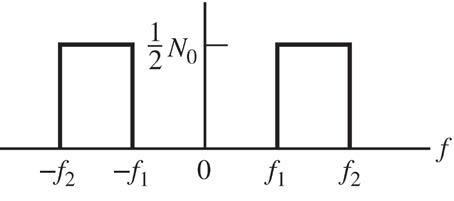
\includegraphics[width=.5\textwidth]{Figure1.jpg}
        \caption{$S_n(f)$}\label{figure1}
    \end{figure}
\end{prob}
\begin{sol}
    The power spectral density of $n(t)$ can be written as
    \begin{align}
        S_n(f)=\frac{N_0}{2}\left[\Pi\left(\frac{f-\frac{f_1+f_2}{2}}{f_2-f_1}\right)+\Pi\left(\frac{f+\frac{f_1+f_2}{2}}{f_2-f_1}\right)\right].
    \end{align}
    \begin{itemize}
        \item[1)] For $f_0=f_1$,
        \begin{align}
            \notag S_{n_c}(f)=S_{n_s}(f)=&\text{LP}[S_n(f-f_0)+S_n(f+f_0)]=\frac{N_0}{2}\left[\Pi\left(\frac{f+\frac{f_2-f_1}{2}}{f_2-f_1}\right)+\Pi\left(\frac{f-\frac{f_2-f_1}{2}}{f_2-f_1}\right)\right]\\
            =&\frac{N_0}{2}\Pi\left(\frac{f}{2(f_2-f_1)}\right),
        \end{align}
        as shown in figure \ref{3-1-1}.
        \begin{align}
            S_{n_cn_s}(f)=j\text{LP}[S_n(f-f_0)-S_n(f+f_0)]=j\frac{N_0}{2}\left[\Pi\left(\frac{f+\frac{f_2-f_1}{2}}{f_2-f_1}\right)-\Pi\left(\frac{f-\frac{f_2-f_1}{2}}{f_2-f_1}\right)\right],
        \end{align}
        as shown in figure \ref{3-1-2}.
        \item[2)] For $f_0=f_2$,
        \begin{align}
            \notag S_{n_c}(f)=S_{n_s}(f)=&\text{LP}[S_n(f-f_0)+S_n(f+f_0)]=\frac{N_0}{2}\left[\Pi\left(\frac{f-\frac{f_2-f_1}{2}}{f_2-f_1}\right)+\Pi\left(\frac{f+\frac{f_2-f_1}{2}}{f_2-f_1}\right)\right]\\
            =&\frac{N_0}{2}\Pi\left(\frac{f}{2(f_2-f_1)}\right),
        \end{align}
        as shown in figure \ref{3-2-1}.
        \begin{align}
            S_{n_cn_s}(f)=j\text{LP}[S_n(f-f_0)-S_n(f+f_0)]=j\frac{N_0}{2}\left[\Pi\left(\frac{f-\frac{f_2-f_1}{2}}{f_2-f_1}\right)-\Pi\left(\frac{f+\frac{f_2-f_1}{2}}{f_2-f_1}\right)\right],
        \end{align}
        as shown in figure \ref{3-2-2}.
        \item[3)] For $f_0=\frac{f_1+f_2}{2}$,
        \begin{align}
            S_{n_c}(f)=S_{n_s}(f)=\text{LP}\left[S_n(f-f_0)+S_n(f+f_0)\right]=N_0\Pi\left(\frac{f}{f_2-f_1}\right),
        \end{align}
        as shown in figure \ref{3-3-1}.
        \begin{align}
            S_{n_cn_s}(f)=j\text{LP}[S_n(f-f_0)-S_n(f+f_0)]=0,
        \end{align}
        as shown in figure \ref{3-3-2}.
        \begin{figure}[h]
            \centering
            \textcolor{red}{There are some mistakes in these figures, please refer to the scan version.}
            \subfigure[$S_{n_c}(f)$ or $S_{n_s}(f)$]{
            \label{3-1-1}
            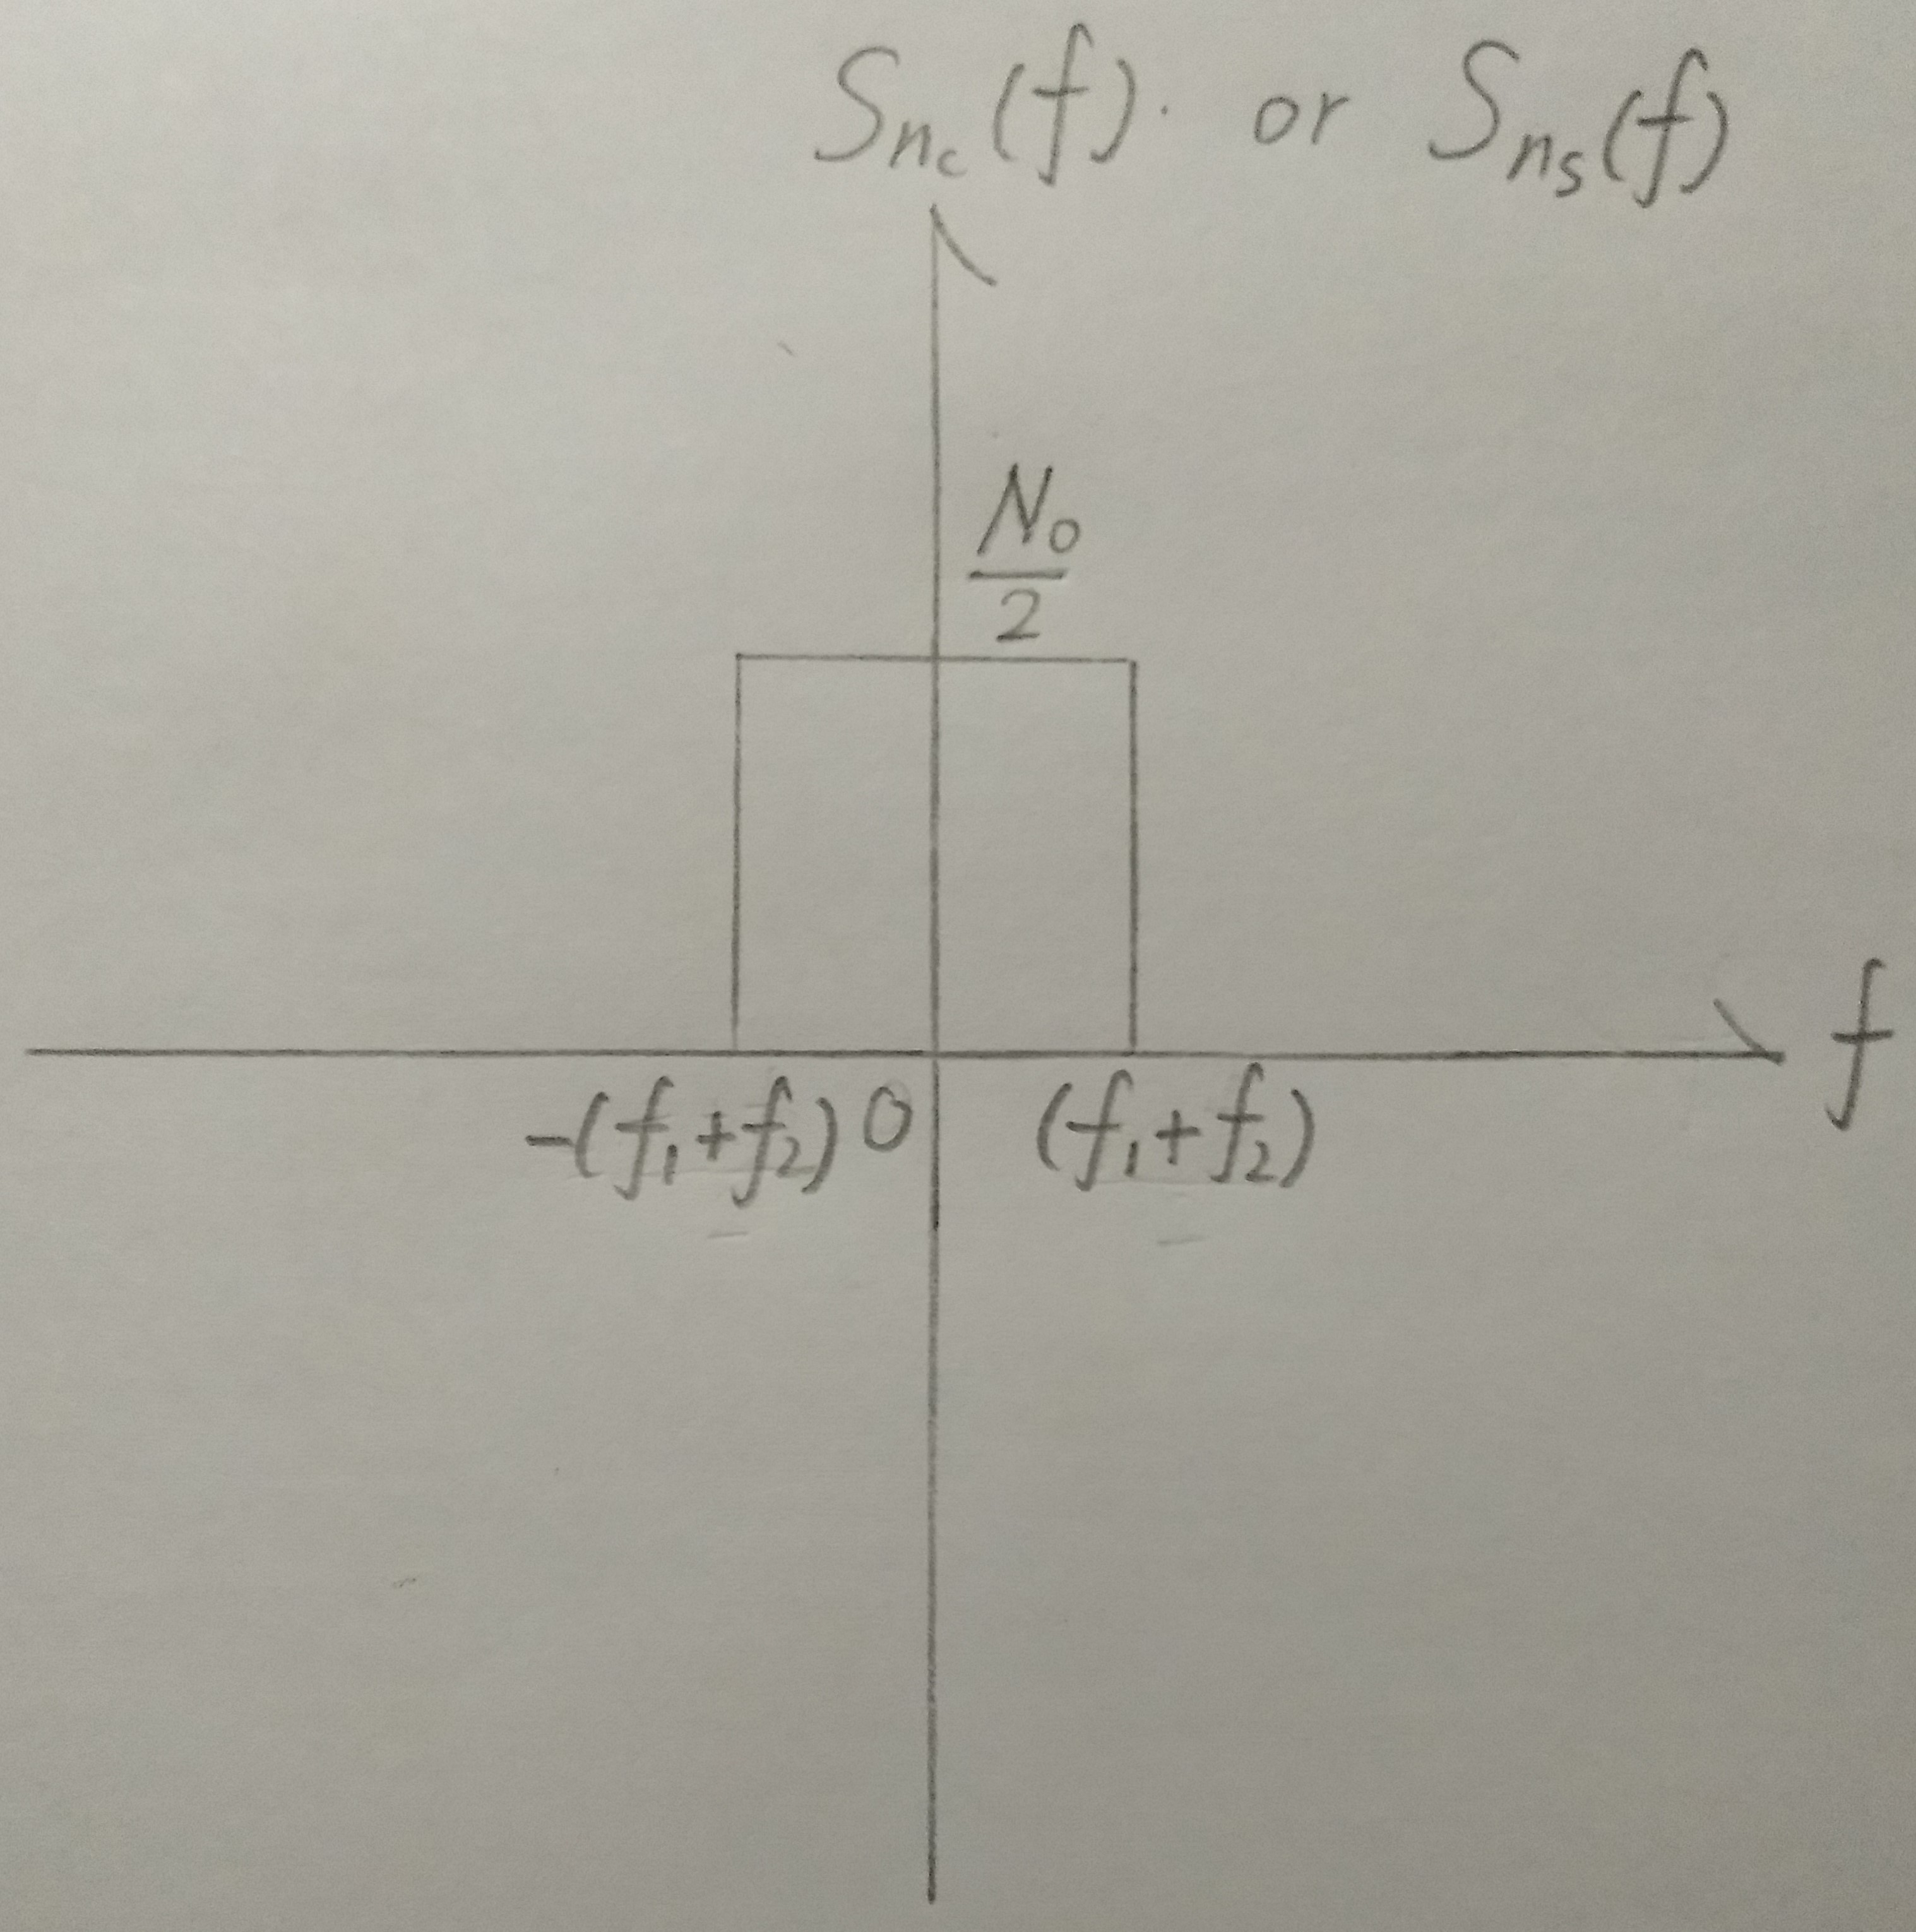
\includegraphics[width=0.35\textwidth]{Assignment-3-Problem-3-1.jpg}}
            \subfigure[$S_{n_cn_s}(f)$]{
            \label{3-1-2}
            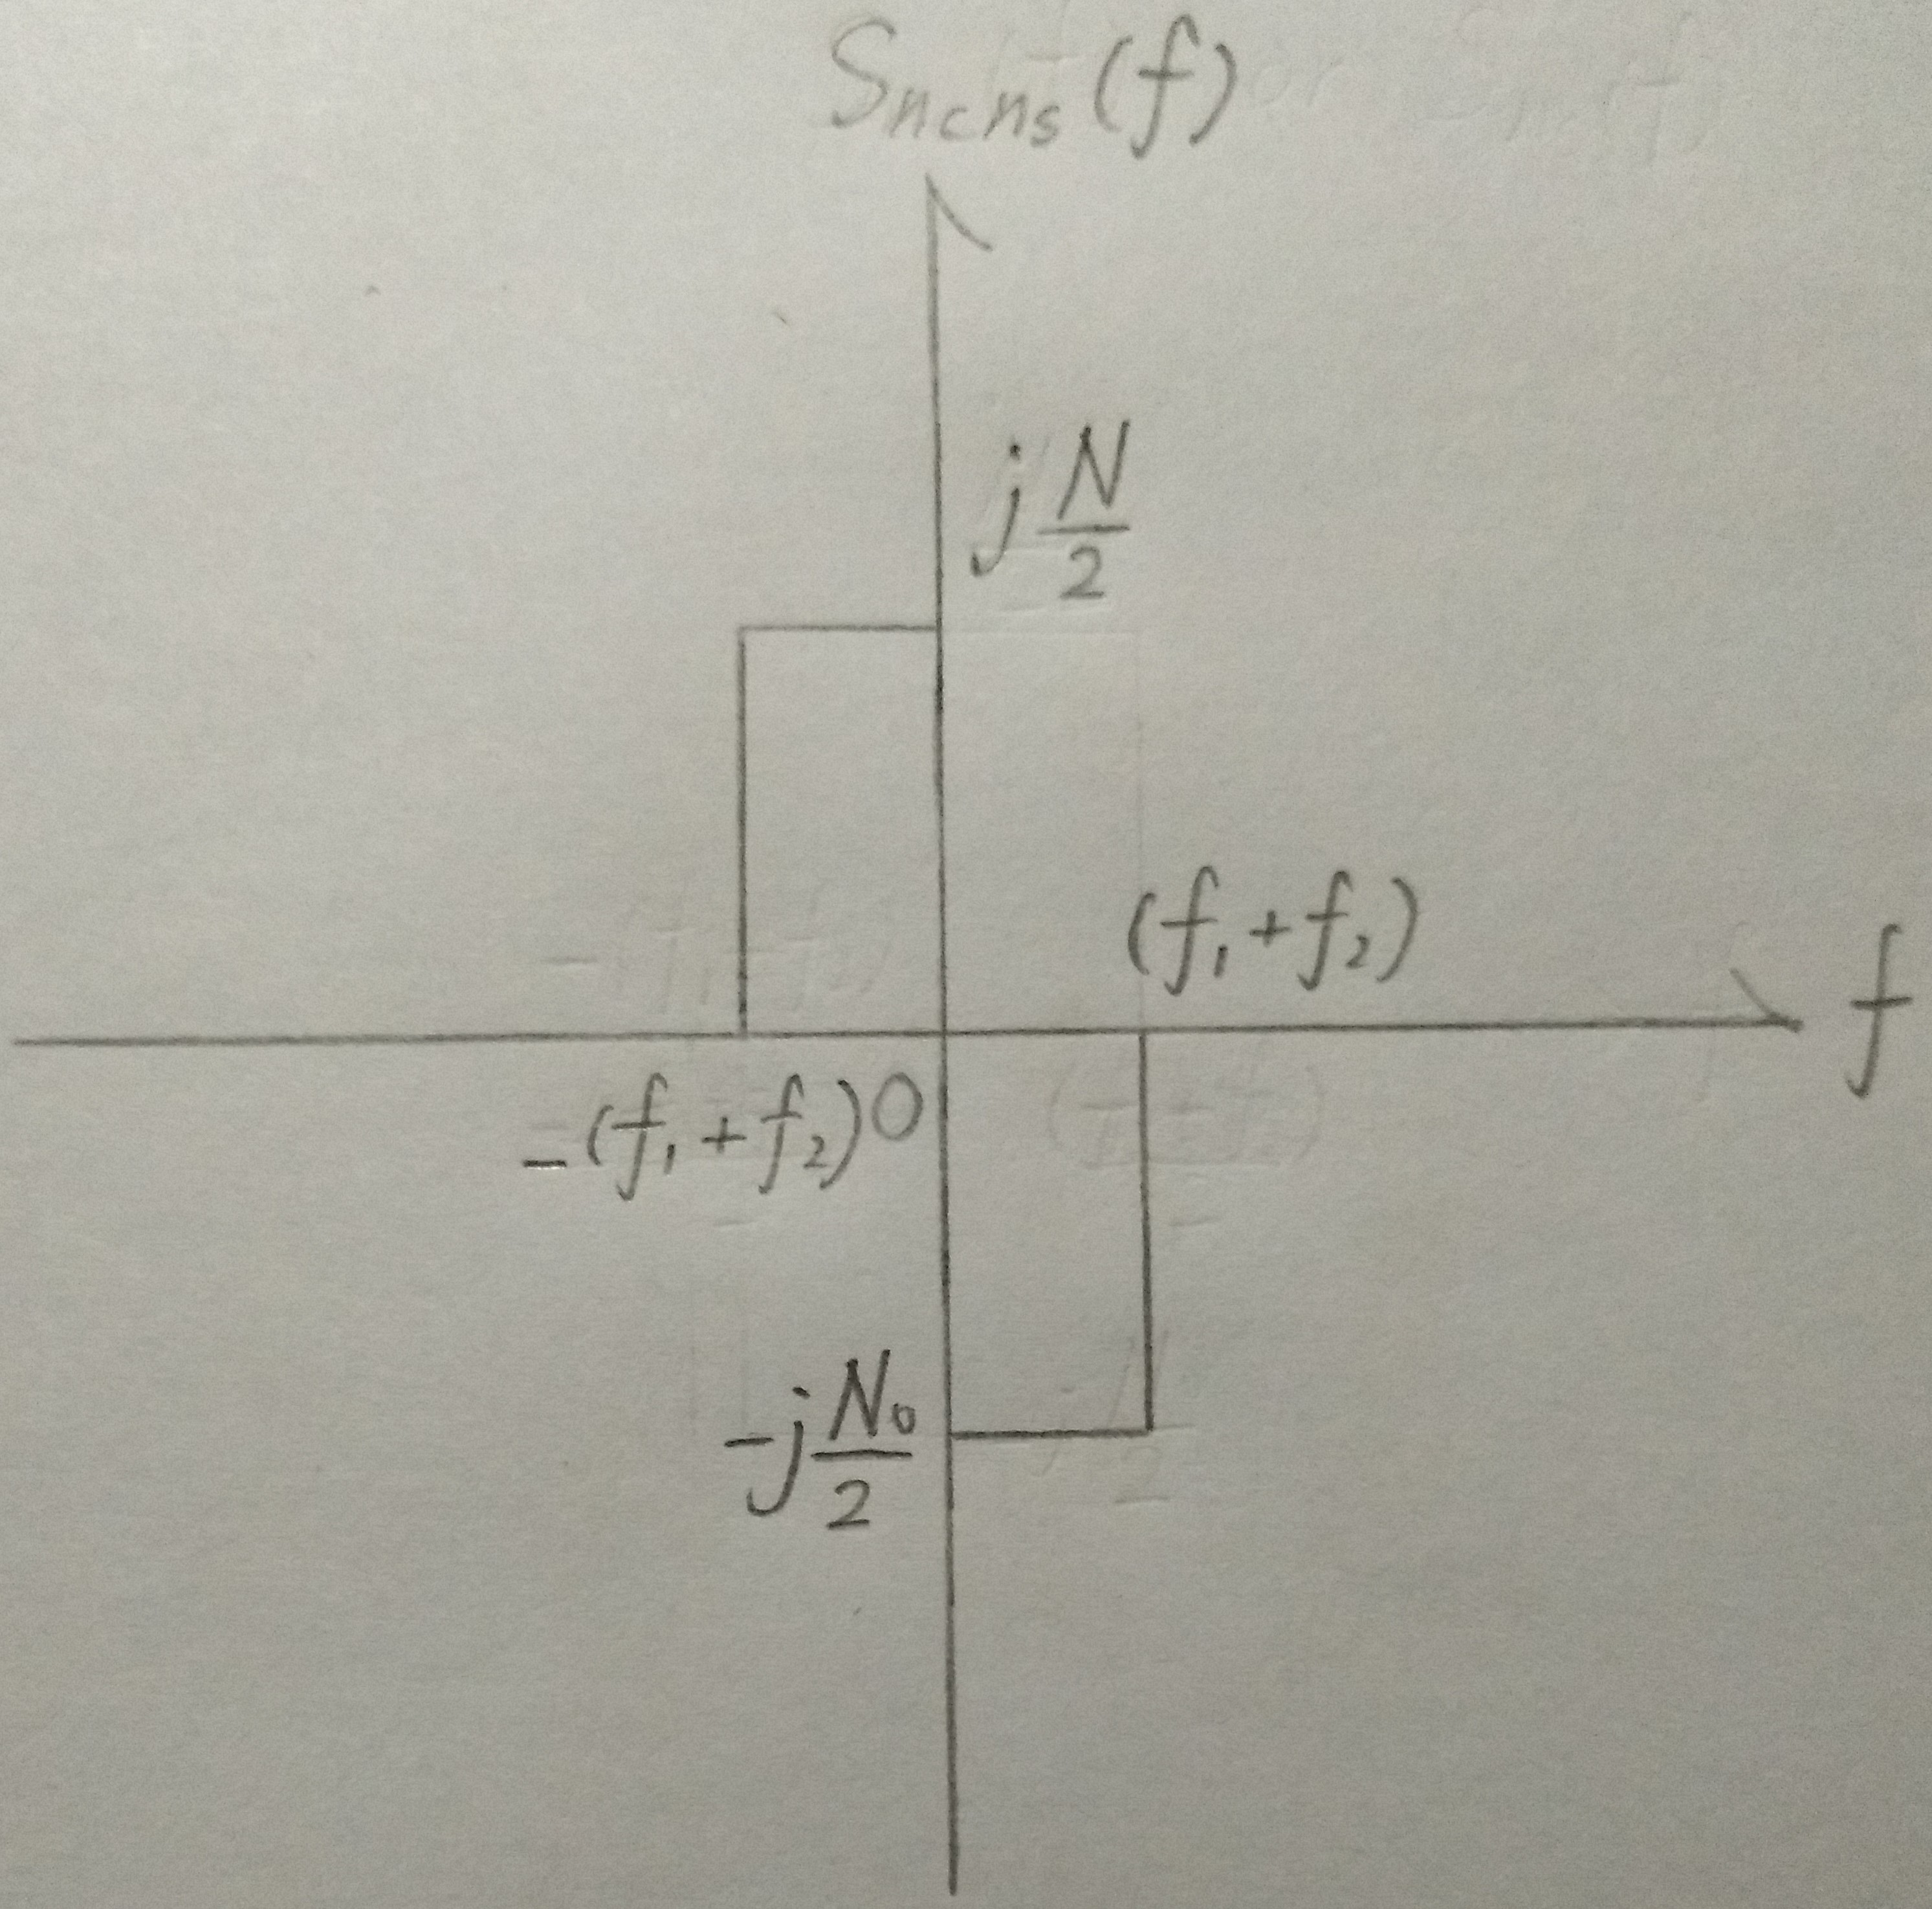
\includegraphics[width=0.35\textwidth]{Assignment-3-Problem-3-2.jpg}}
            \caption{Case 1)}
            \subfigure[$S_{n_c}(f)$ or $S_{n_s}(f)$]{
            \label{3-2-1}
            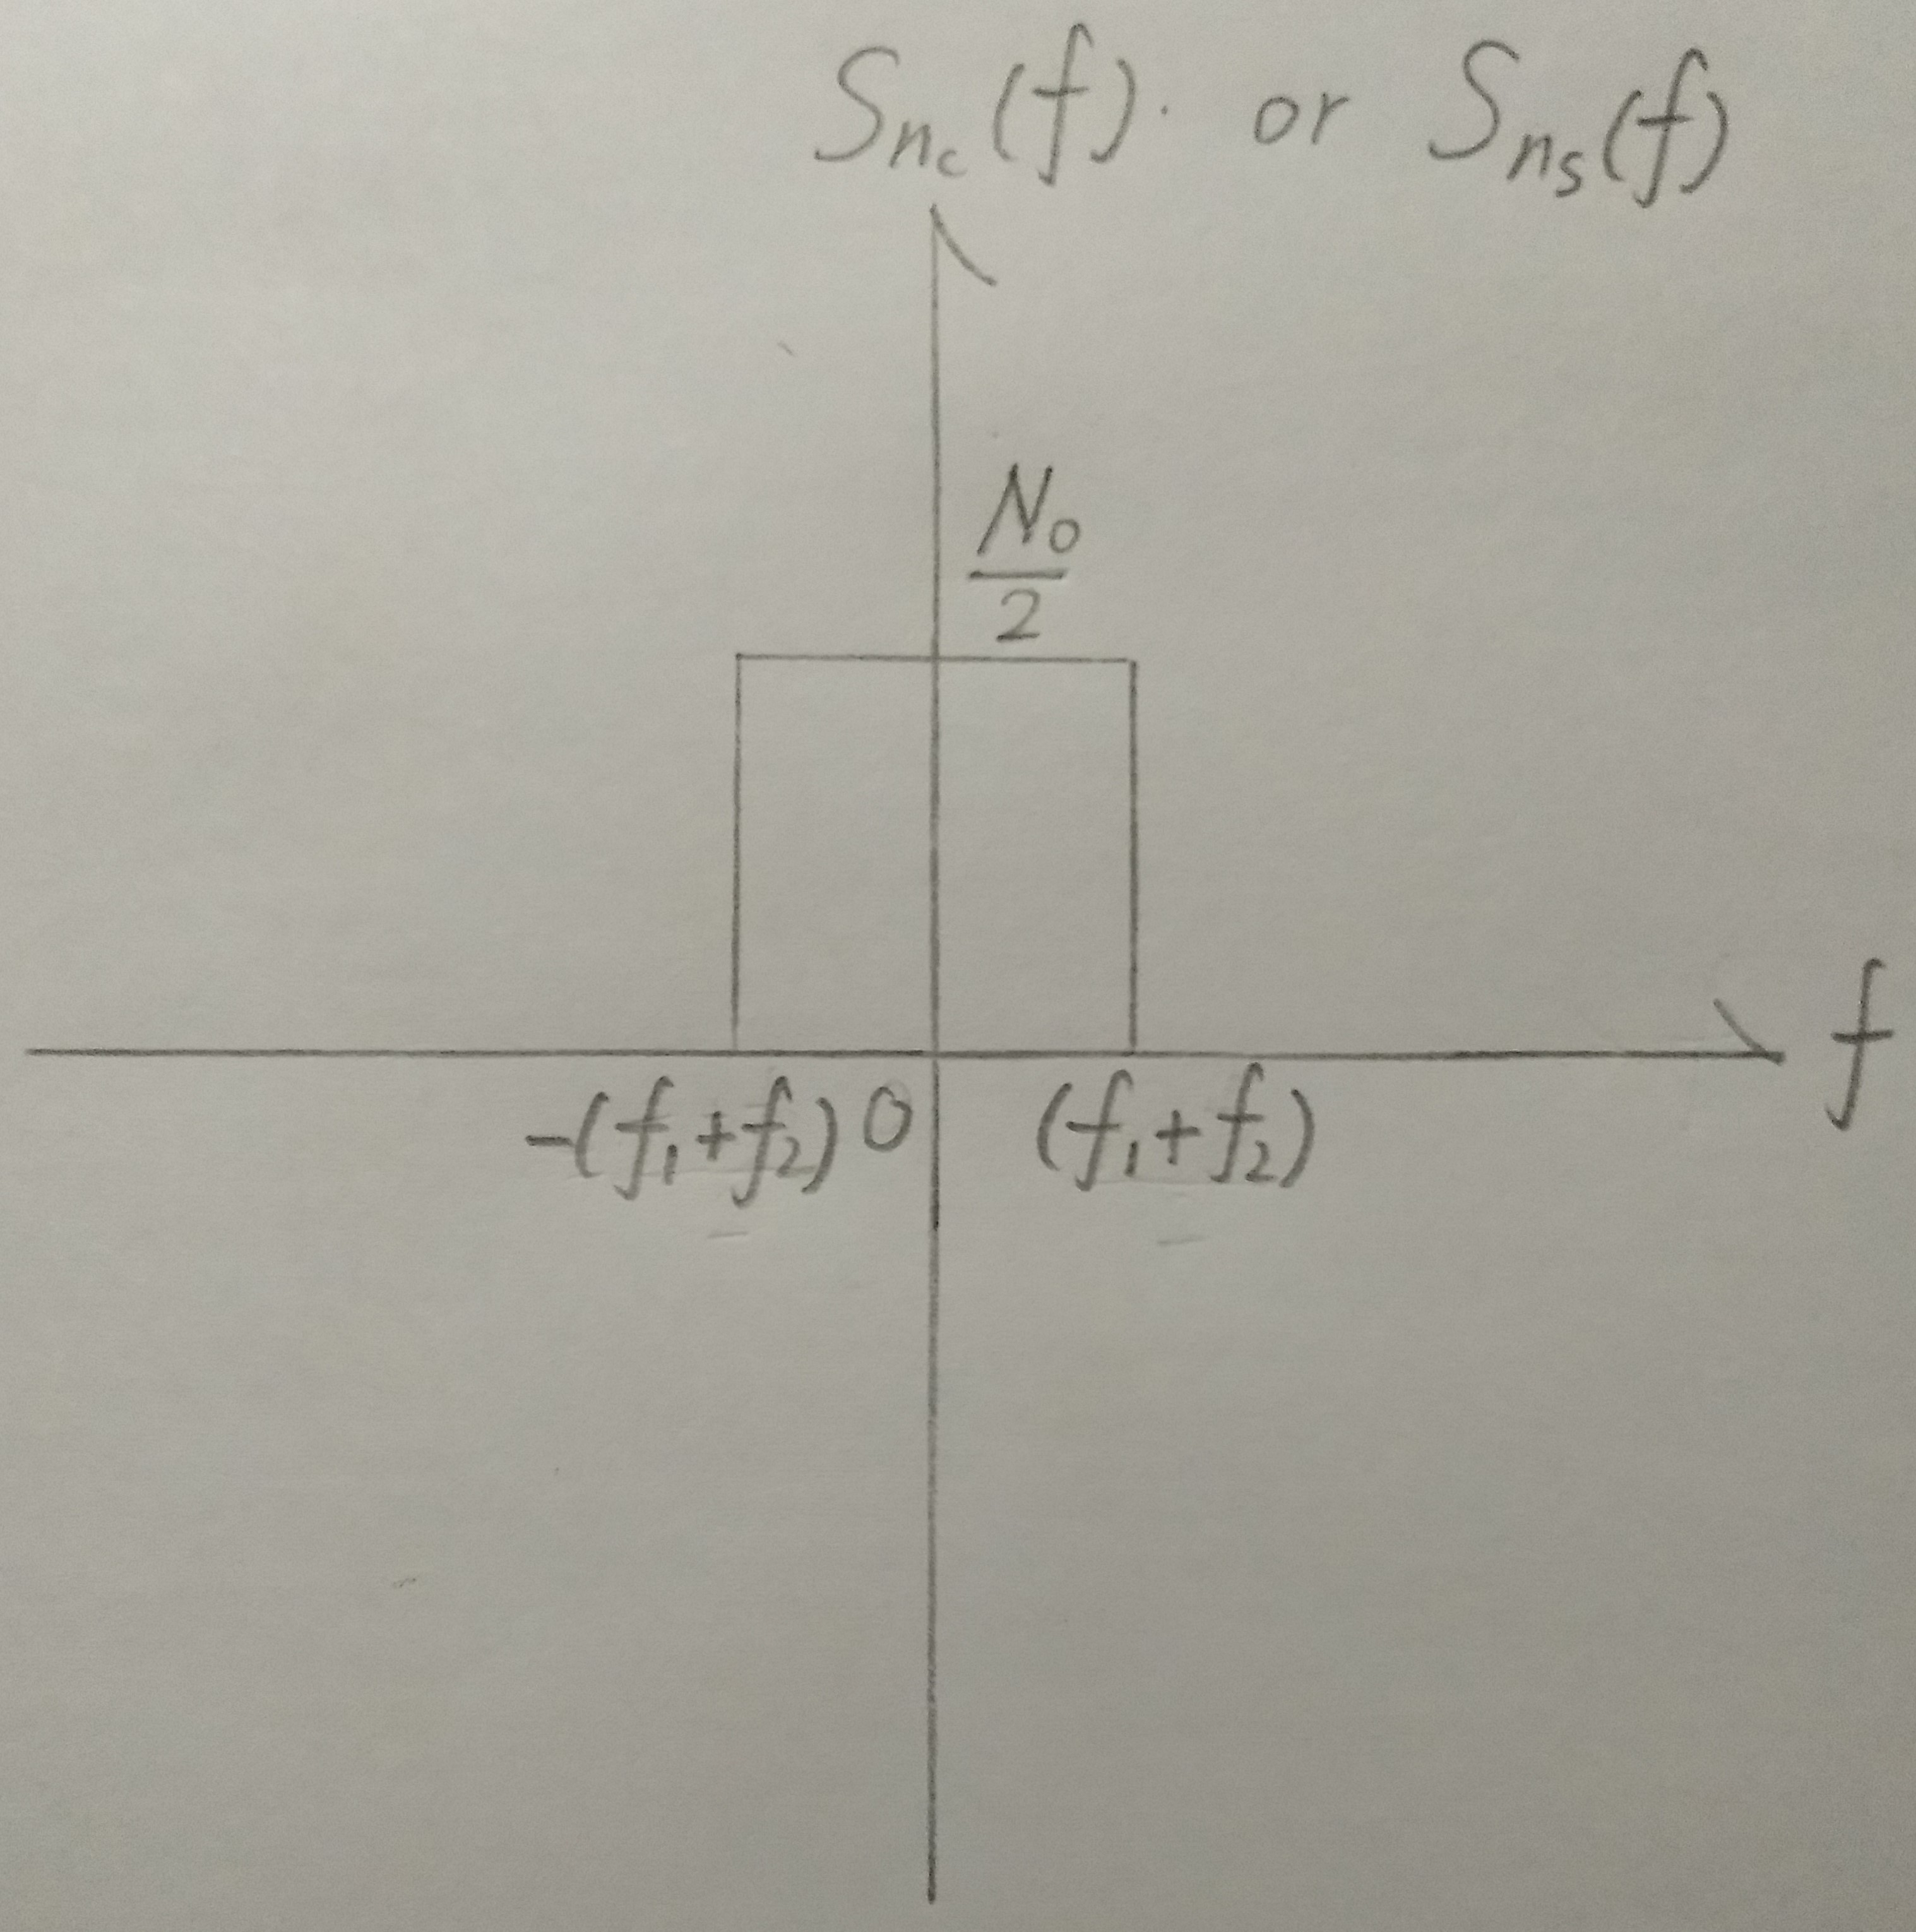
\includegraphics[width=0.35\textwidth]{Assignment-3-Problem-3-1.jpg}}
            \subfigure[$S_{n_cn_s}(f)$]{
            \label{3-2-2}
            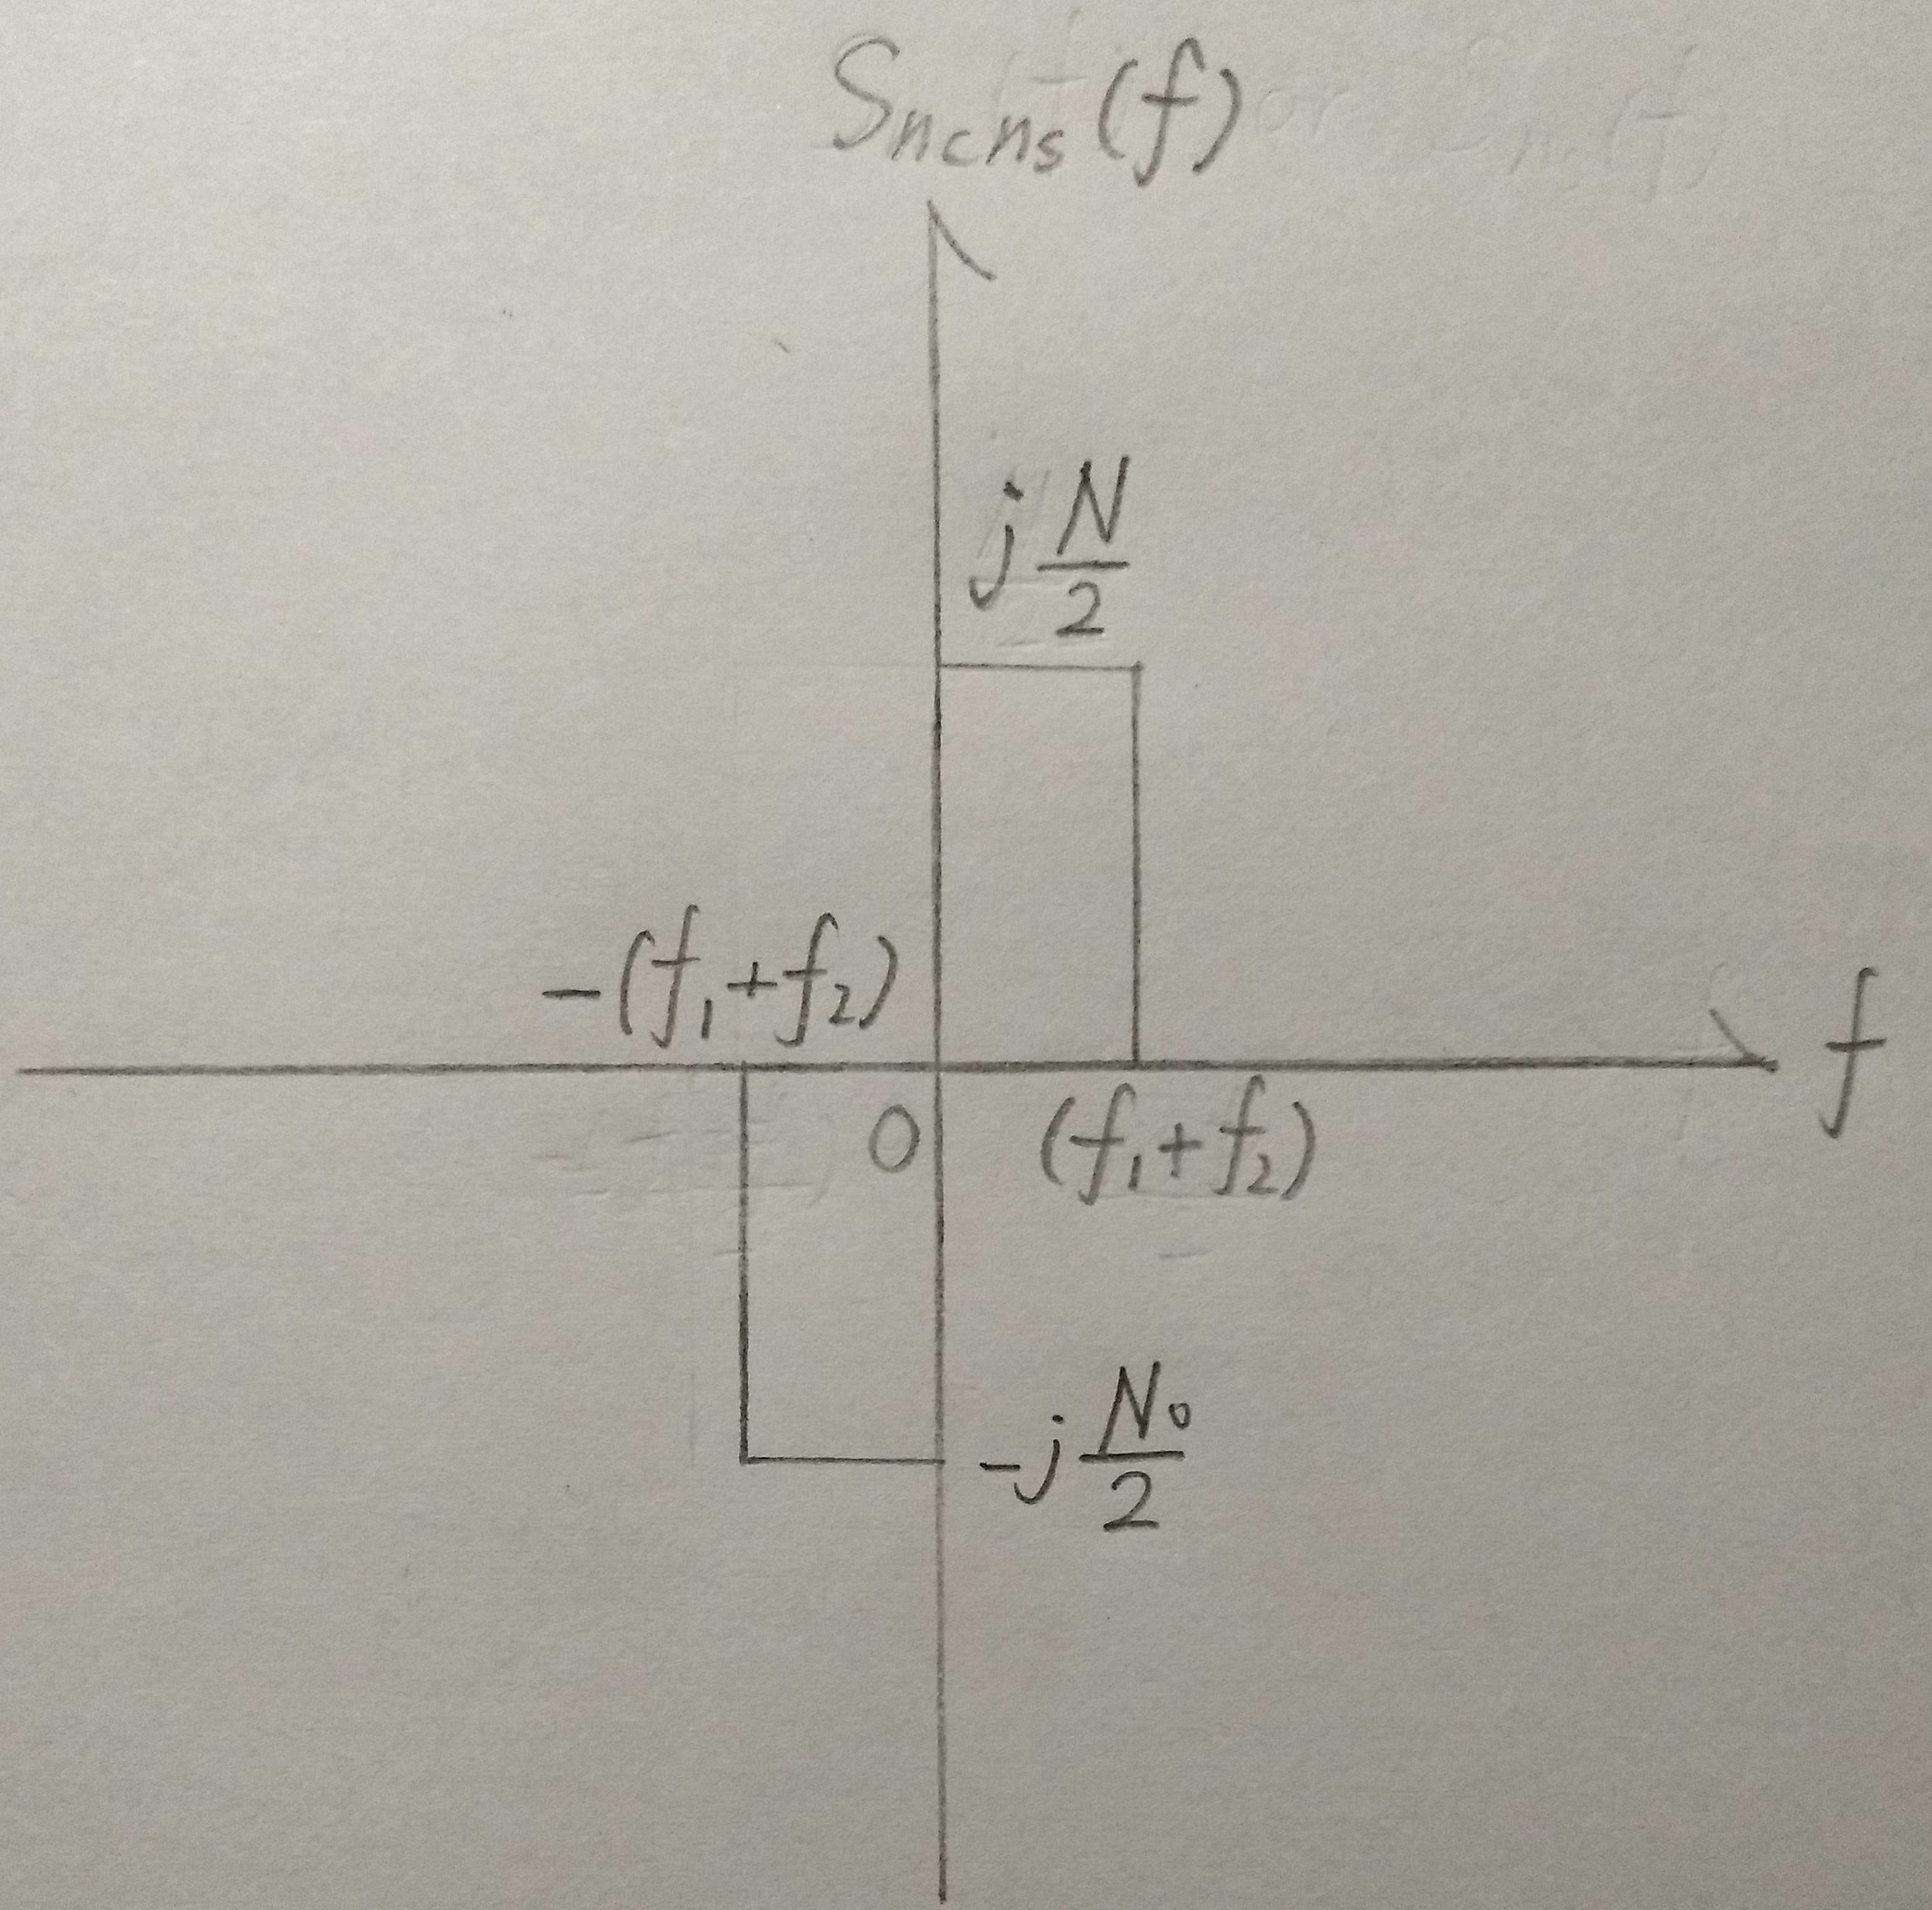
\includegraphics[width=0.35\textwidth]{Assignment-3-Problem-3-3.jpg}}
            \caption{Case 2)}
            \subfigure[$S_{n_c}(f)$ or $S_{n_s}(f)$]{
            \label{3-3-1}
            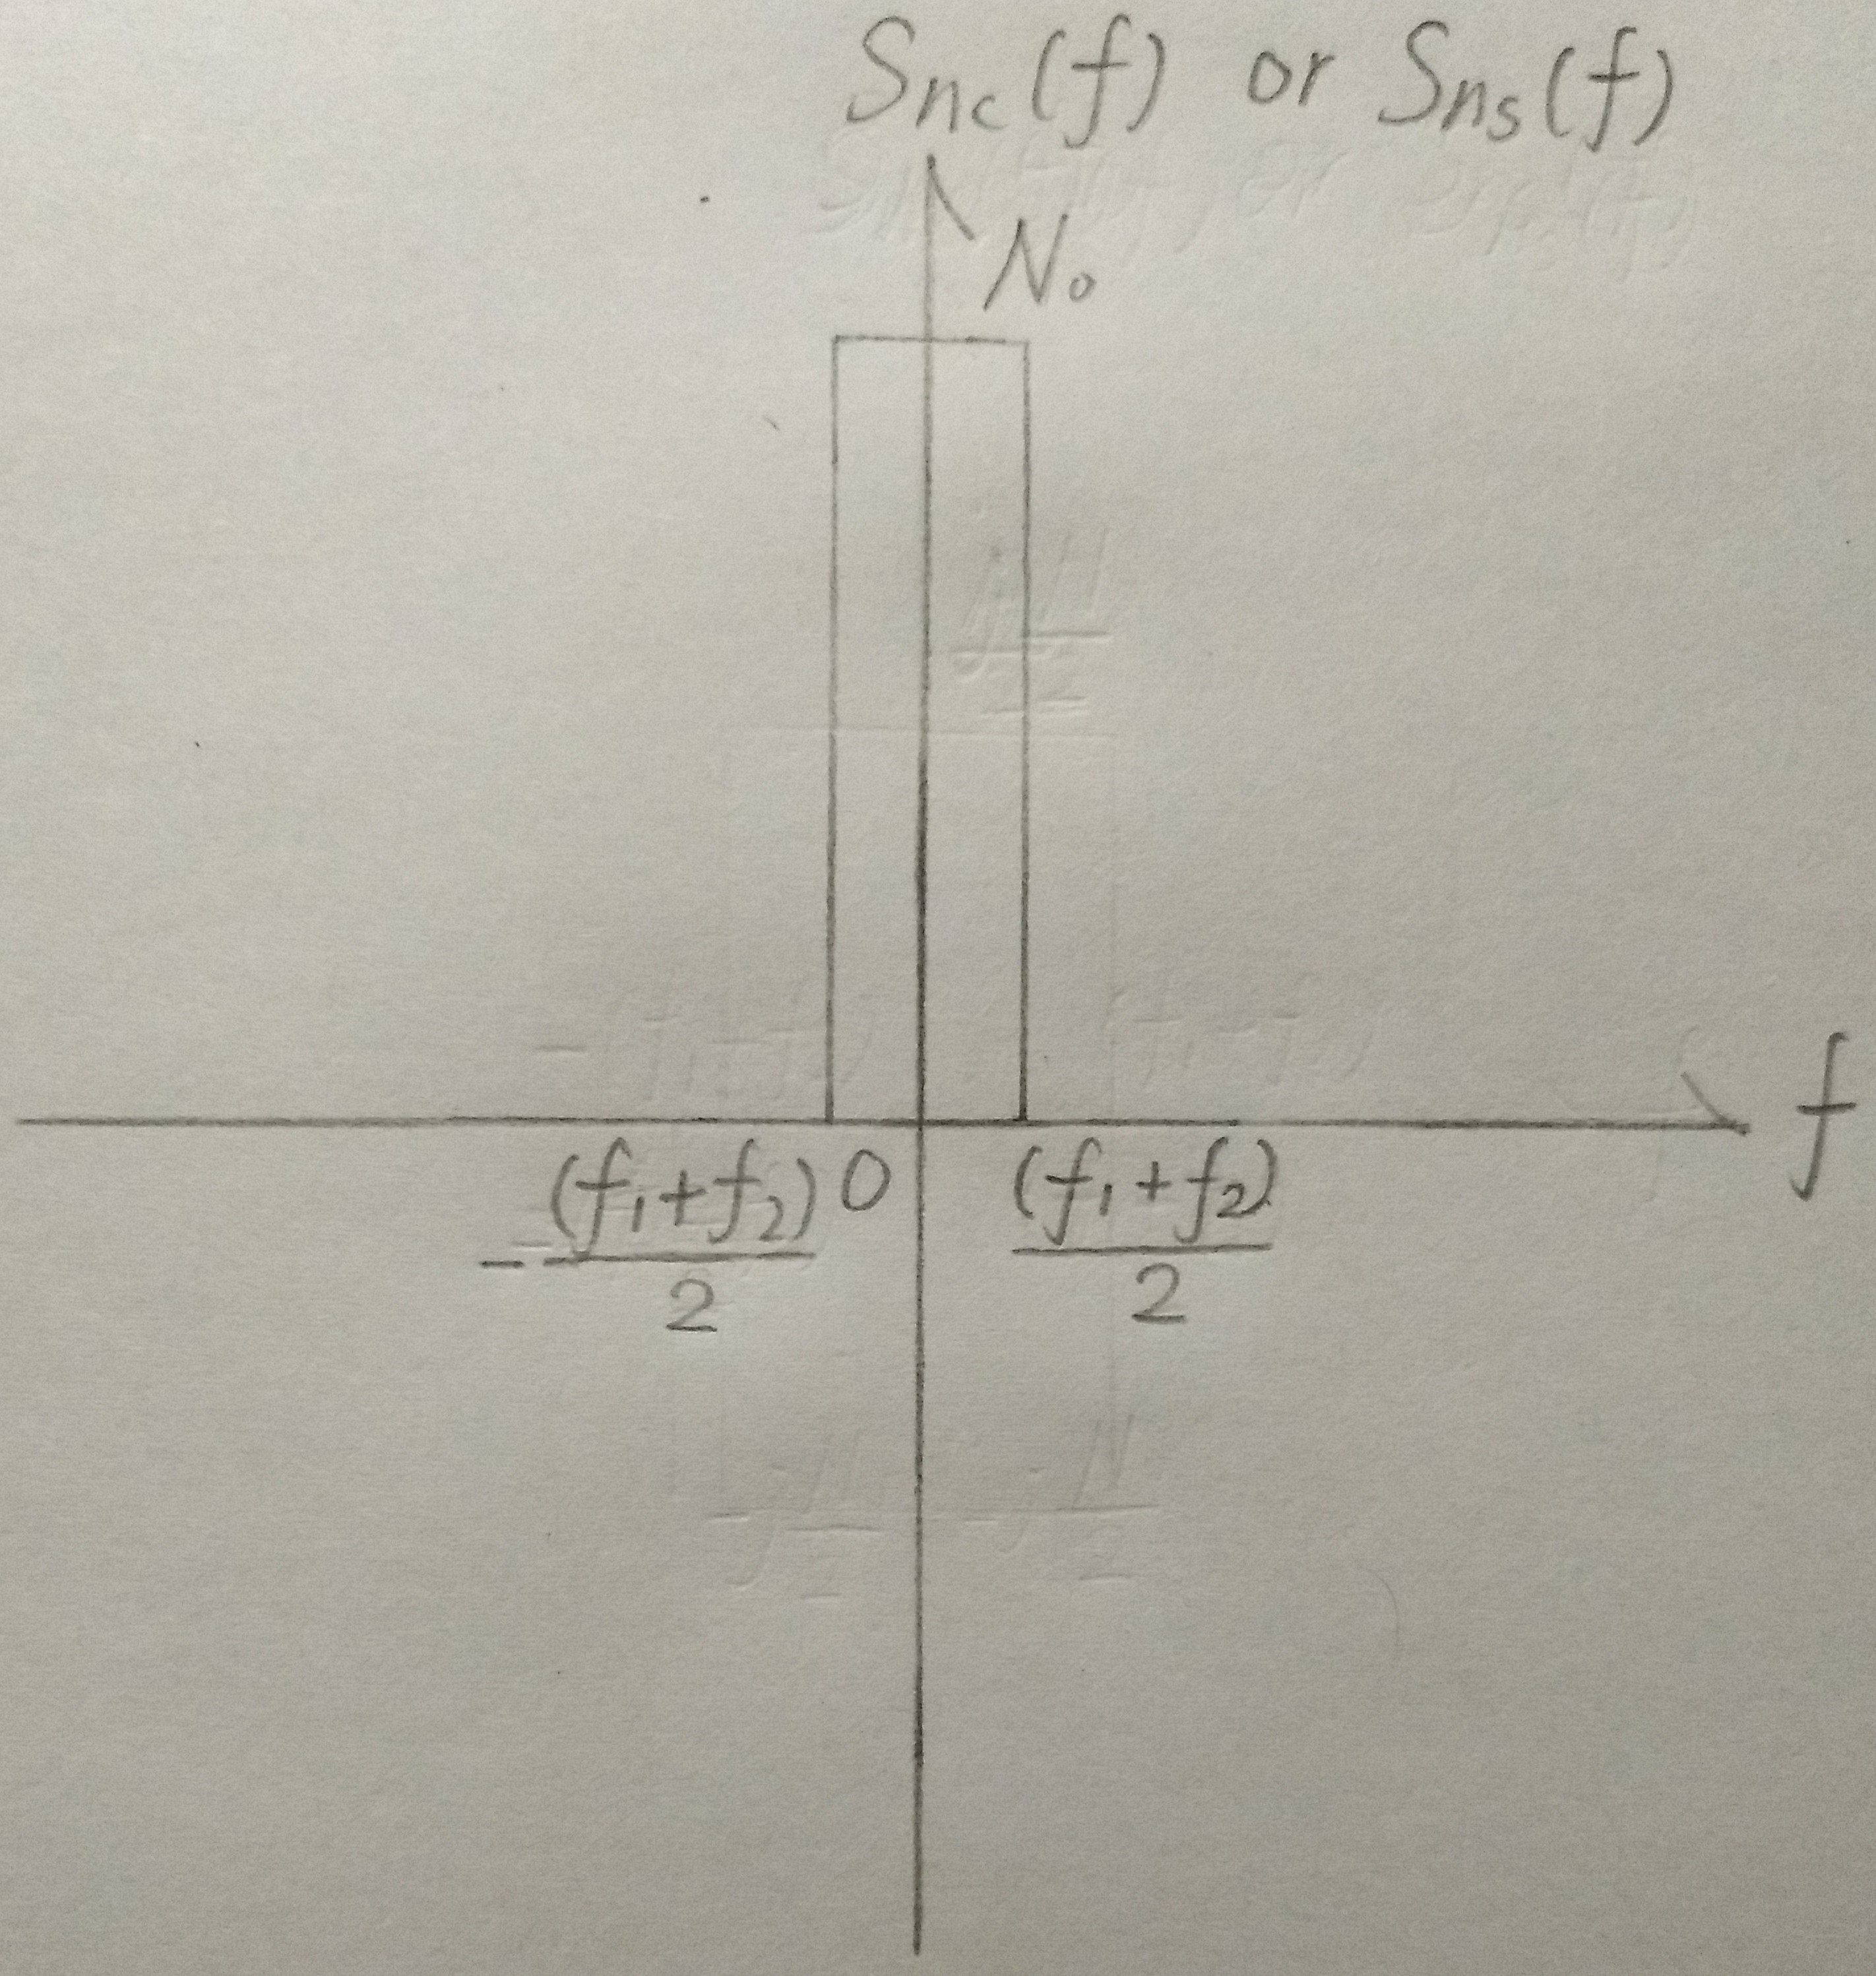
\includegraphics[width=0.35\textwidth]{Assignment-3-Problem-3-4.jpg}}
            \subfigure[$S_{n_cn_s}(f)$]{
            \label{3-3-2}
            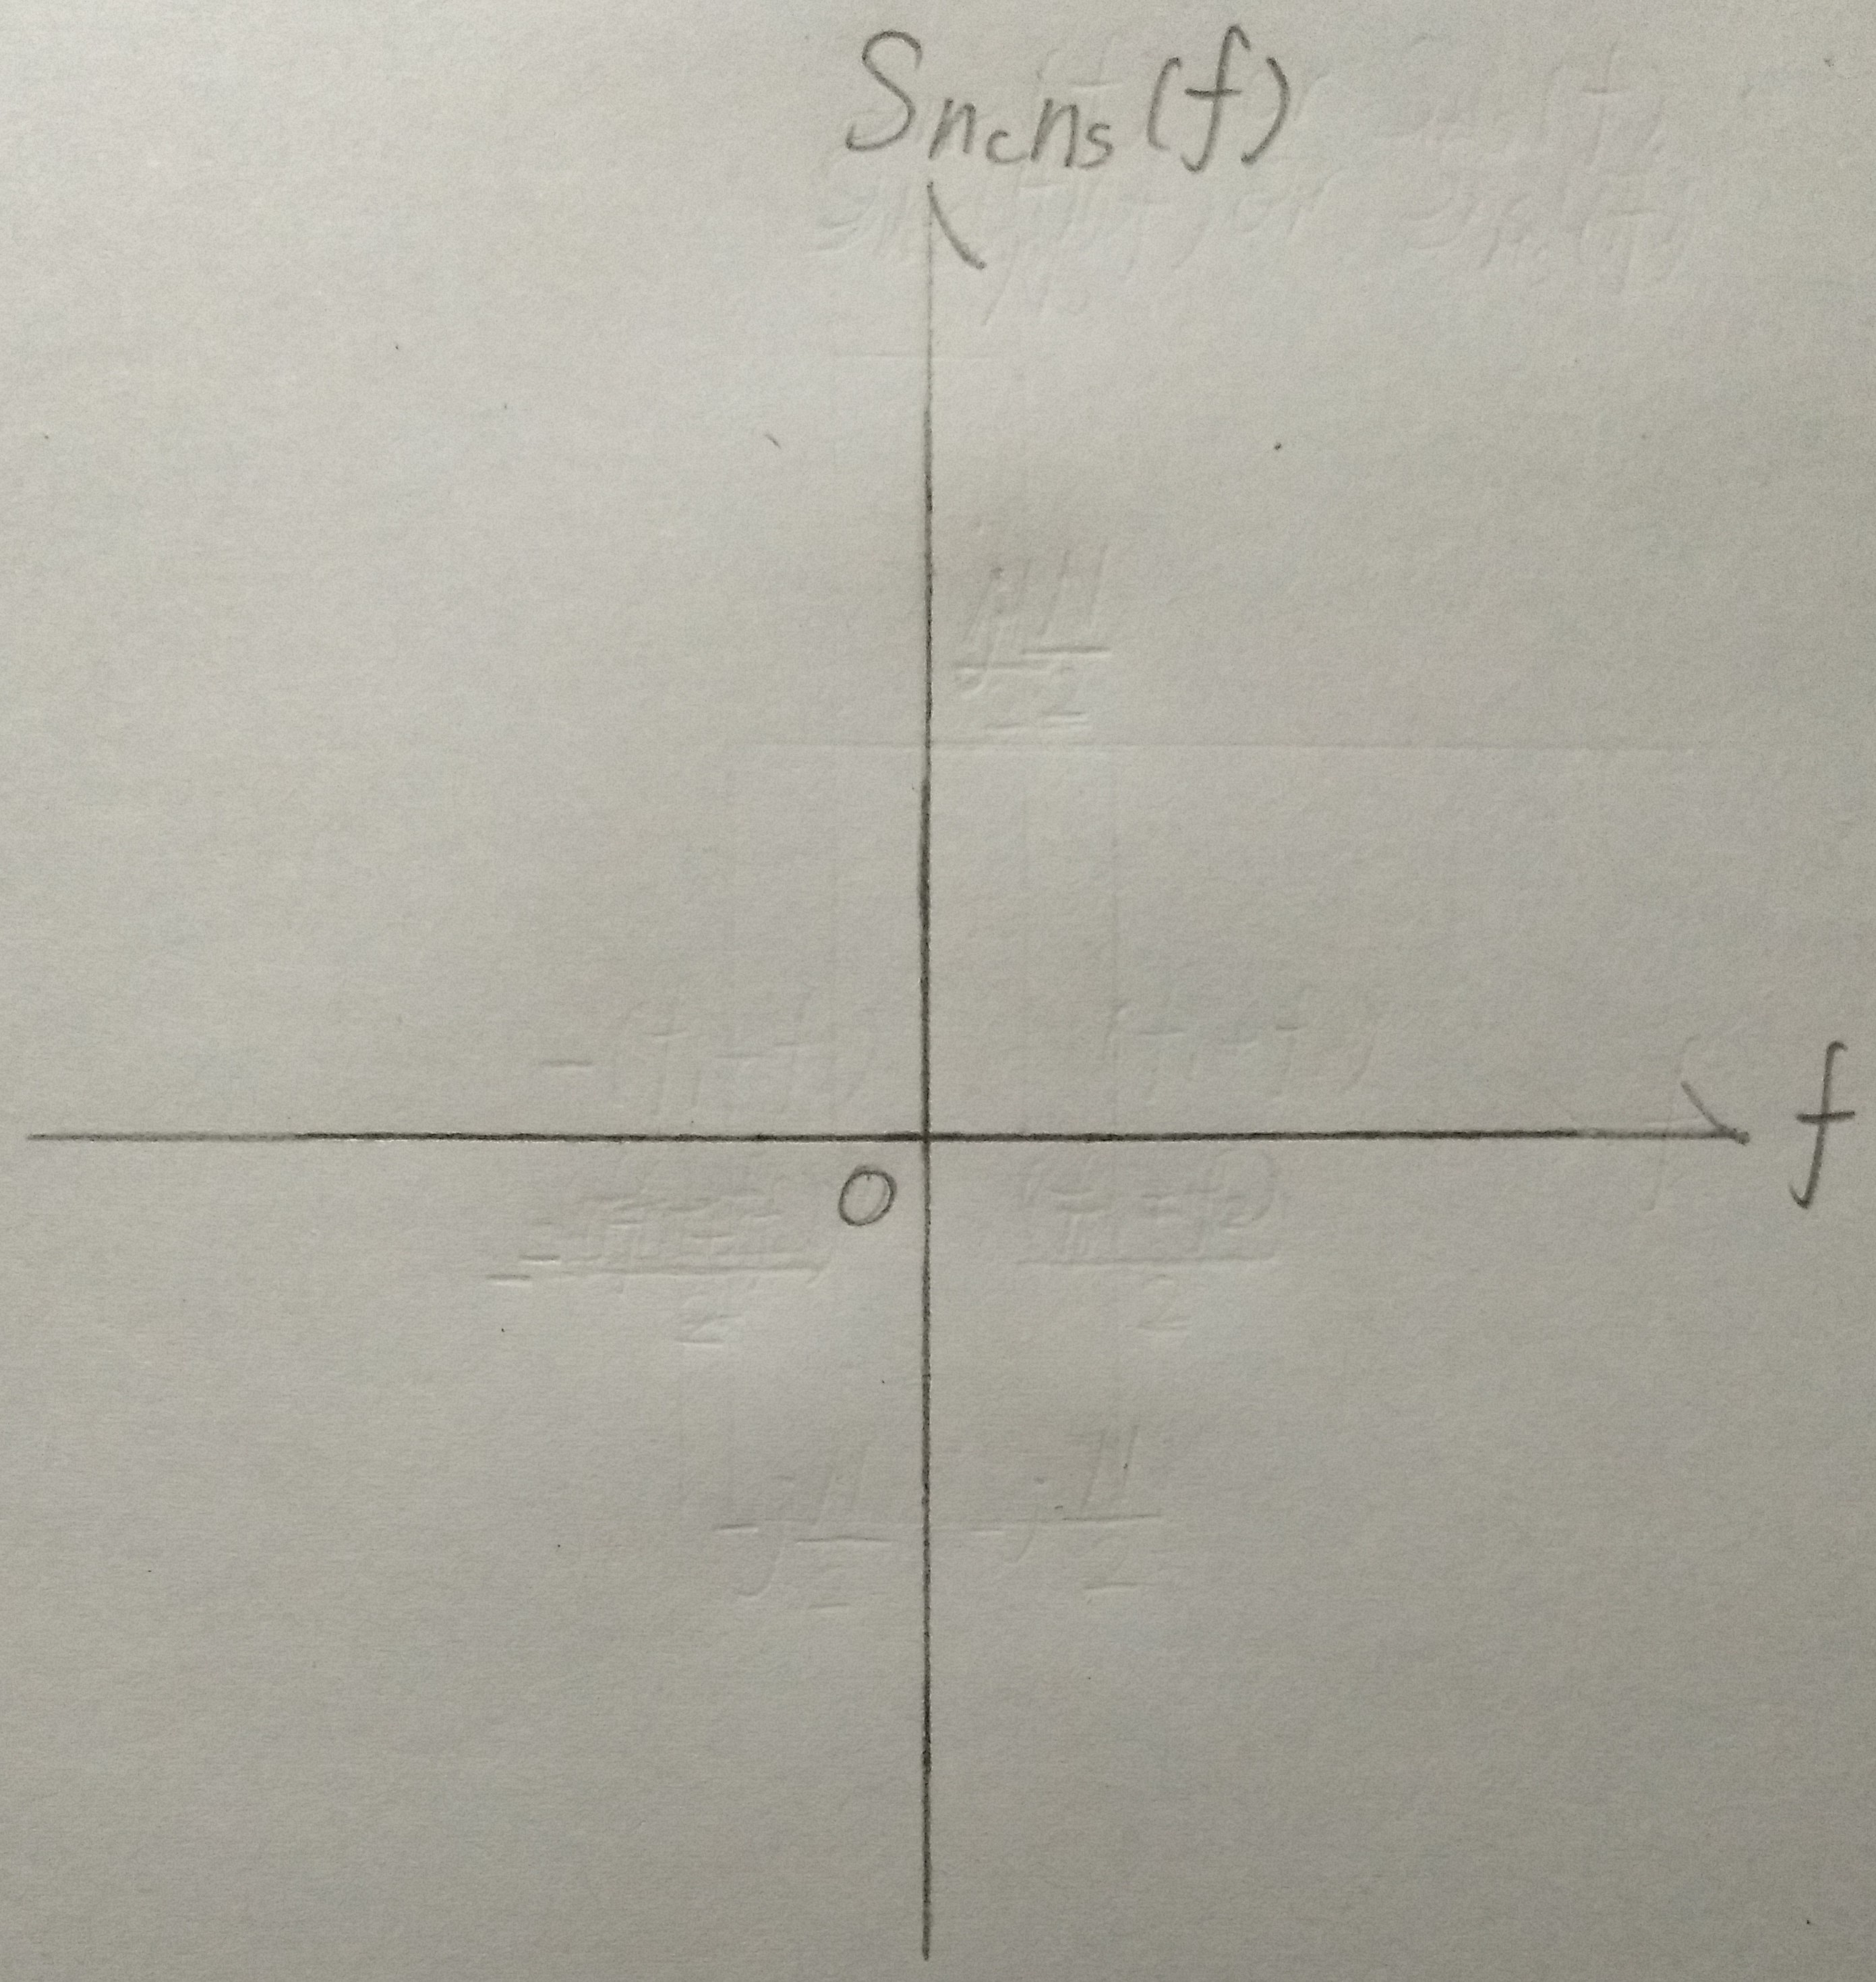
\includegraphics[width=0.35\textwidth]{Assignment-3-Problem-3-5.jpg}}
            \caption{Case 3)}
        \end{figure}
        \item[4)] \sout{For cases \textbf{1), 2) and 3)}, $n_c(t)$ and $n_s(t)$ are uncorrelated. This is because, for all the cases above, the cross power spectral density is pure imaginary, so that the correlation function of $n_s(t)$ and $n_c(t)$, $R_{n_sn_c}(\tau)=\mathscr{F}^{-1}[S_{n_sn_c}(f)]$, is an odd function and thus $R_{n_sn_c}(0)=0$. Therefore, for all the cases above, $n_c(t)$ and $n_s(t)$ are uncorrelated.}\\
        \textcolor{red}{Only in case 3), $n_c(t)$ and $n_s(t)$ are uncorrelated, since only in case 3), $R_{n_sn_c}(t)=\mathscr{F}^{-1}[S_{n_sn_c}(f)]=0\quad\forall\tau$. In case 1) and 2), $R_{n_sn_c}(\tau)=\mathscr{F}^{-1}[S_{n_sn_c}(f)]=\pm\frac{N_0}{2}(f_2-f_1)\sinc[(f_2-f_1)\tau]e^{-j2\pi\frac{f_2-f_1}{2}\tau}\mp\frac{N_0}{2}(f_2-f_1)\sinc[(f_2-f_1)\tau]e^{+j2\pi\frac{f_2-f_1}{2}\tau}=\pm N_0\pi(f_2-f_1)^2\tau\sinc^2[(f_2-f_1)\tau]=0$ only for $\tau=\frac{m}{f_2-f_1}$, $m=0,\pm 1,\pm 2,\cdots$}
    \end{itemize}
\end{sol}
\end{document}